\begin{frame}
    \frametitle{Radiation Modeling}
    Solar radiation received by a surface can be divided into direct (B), diffuse (D), and reflected (R) components. The sum of these components is the  global radiation (G).
    \vspace*{0.5cm}
    \begin{figure}
        \centering
        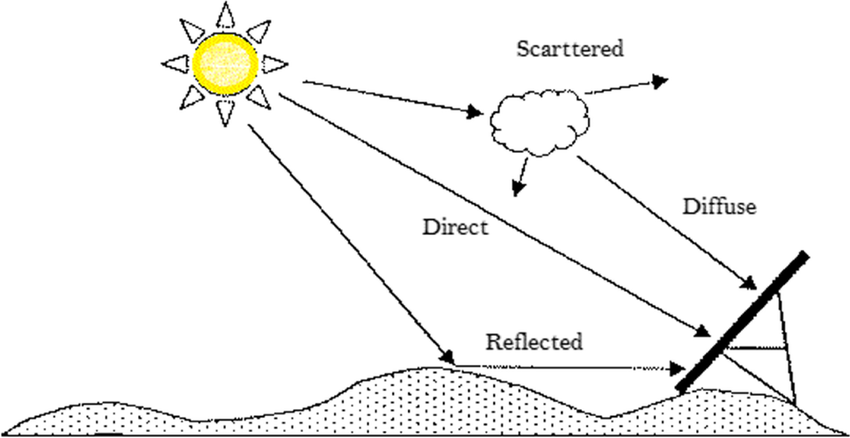
\includegraphics{Radiation_components.png}
        \caption{\small Illustration of solar radiation components received by a surface.}
        \label{fig:radiation_components}
    \end{figure}
\end{frame}